\section{Evaluation}
\begin{frame}
    \frametitle{Vergleich}
    \begin{table}[]
    \centering
    \begin{tabular}{|l|l|l|l|}
    \hline
    m=n                    & H Methode & s-H Methode & Verbesserung \\\hline
    FSBRTS                 & 511       & 337         & 34 \%        \\
    Synthetic              & 61        & 31          & 49 \%        \\
    Garage Door Controller & 13        & 13          & 0 \%         \\
    \hline
    \end{tabular}
    \end{table}
    \end{frame}
    
    \begin{frame}
    \frametitle{Beispiel: Garage Door Controller}
    Fernbedienung mit einer Taste steuert Garagentür
    Garagentür kann:
    \begin{itemize}
        \item herunterfahren
        \item hochfahren
        \item stoppen
        \item Richtung wechseln
        \item Lichtschranke aktivieren und stoppen
    \end{itemize}
    
    \end{frame}
    \begin{frame}
    \frametitle{Beispiel: Garage Door Controller}
    \centering
    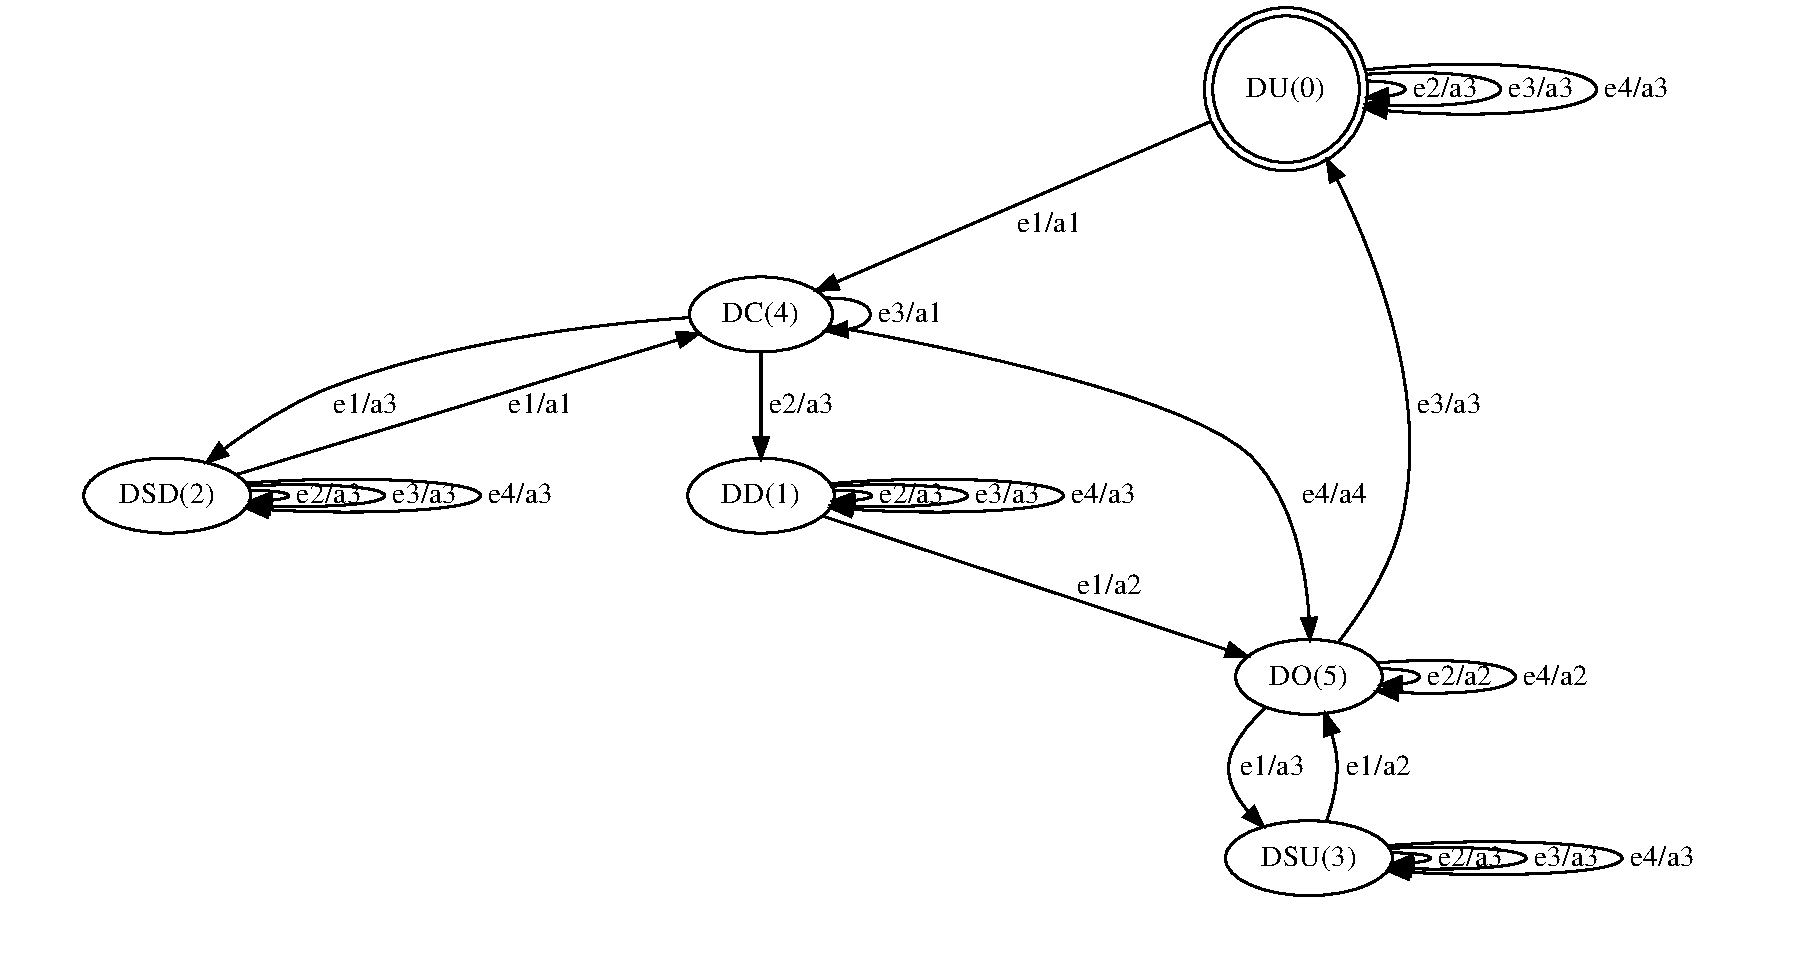
\includegraphics[width=1.15\textwidth]{images/gdc}
    
    \end{frame}
    
    
    \begin{frame}
    \frametitle{Beispiel: Garage Door Controller}
    \begin{columns}[T] % align columns
    \begin{column}{.55\textwidth}
    
    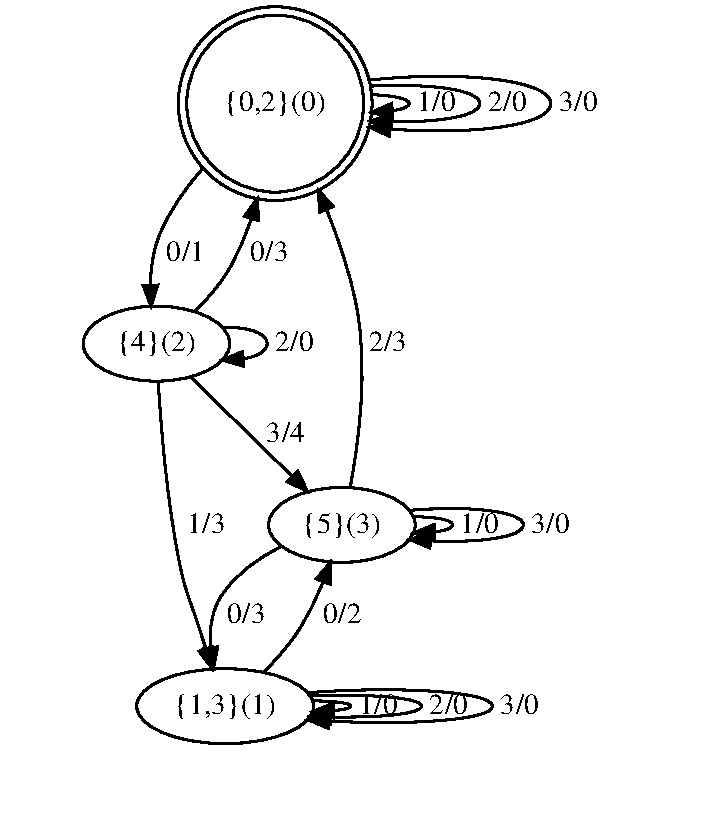
\includegraphics[width=\textwidth]{images/gdc_min}
    \end{column}%
    \hfill%
    \begin{column}{.55\textwidth}
    Eingabe:
    \begin{itemize}
      \item e1: Fernbedienung gedrückt
      \item e2: Sensor "Tür ist unten"
      \item e3: Sensor "Tür ist oben"
      \item e4: Sensor "Lichtschrank aktiviert"
    \end{itemize}
    Ausgabe:
    \begin{itemize}
      \item a1: "Tür fährt herunter"
      \item a2: "Tür fährt hoch"
      \item a3: "Stop"
      \item a4: "Richtungswechsel unten $\rightarrow$ oben"
    \end{itemize}
    \end{column}%
    \end{columns}
    \end{frame}
    
    \begin{frame}
    \frametitle{Beispiel: Garage Door Controller}
    \begin{columns}[T] % align columns
    \begin{column}{.55\textwidth}
    
    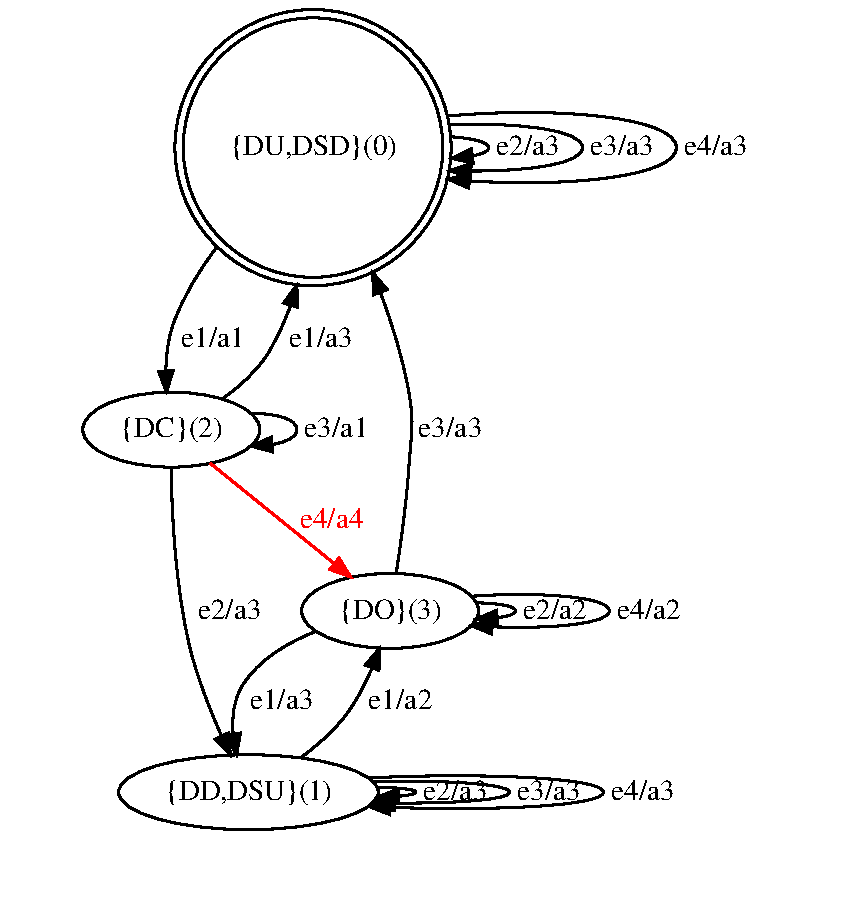
\includegraphics[width=\textwidth]{images/gdc_min_colored}
    \end{column}%
    \hfill%
    \begin{column}{.55\textwidth}
    Eingabe:
    \begin{itemize}
      \item e1: Fernbedienung gedrückt
      \item e2: Sensor "Tür ist unten"
      \item e3: Sensor "Tür ist oben"
      \item e4: Sensor "Lichtschrank aktiviert"
    \end{itemize}
    Ausgabe:
    \begin{itemize}
      \item a1: "Tür fährt herunter"
      \item a2: "Tür fährt hoch"
      \item a3: "Stop"
      \item a4: "Richtungswechsel unten $\rightarrow$ oben"
    \end{itemize}
    Sicherheitskritisch ist nur \textcolor{red}{a4}.
    \end{column}%
    \end{columns}
    \end{frame}
    
    \begin{frame}
    \frametitle{Beispiel: Garage Door Controller}
    \begin{columns}[T] % align columns
    \begin{column}{.53\textwidth}
    
    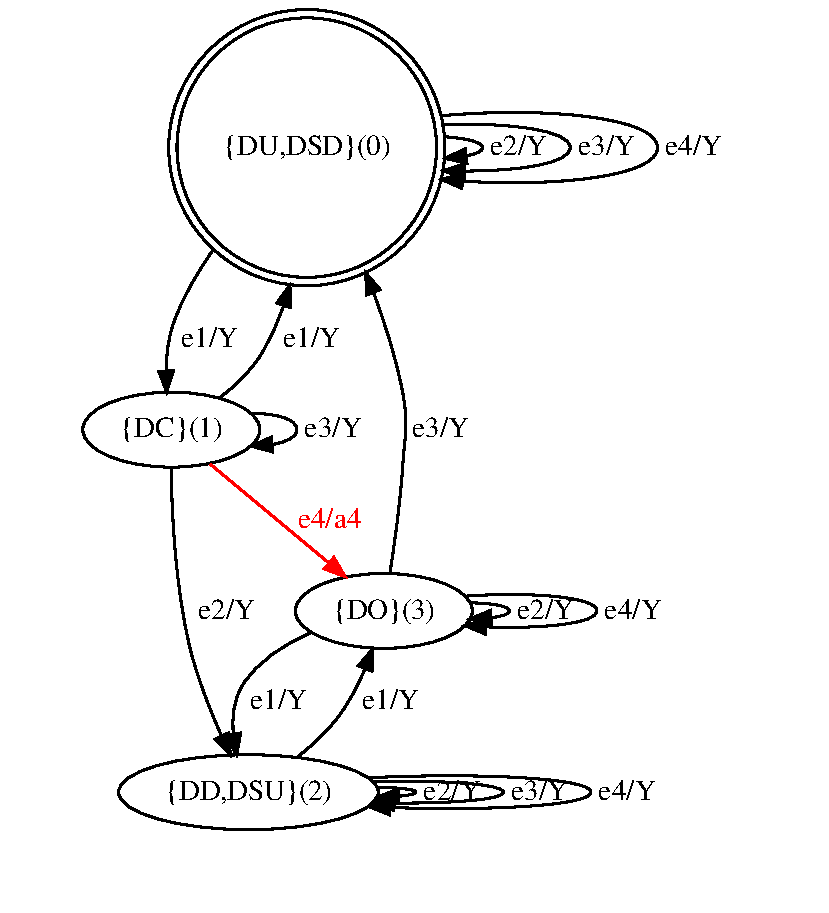
\includegraphics[width=\textwidth]{images/gdc_abs_min_colored}
    \end{column}%
    \hfill%
    \begin{column}{.55\textwidth}
    Eingabe:
    \begin{itemize}
      \item e1: Fernbedienung gedrückt
      \item e2: Sensor "Tür ist unten"
      \item e3: Sensor "Tür ist oben"
      \item e4: Sensor "Lichtschrank aktiviert"
    \end{itemize}
    Ausgabe:
    \begin{itemize}
      \item a4: "Richtungswechsel unten $\rightarrow$ oben"
      \item Y: Sonstige
    \end{itemize}
    Sicherheitskritisch ist nur \textcolor{red}{a4}.
    \end{column}%
    \end{columns}
    \end{frame}